\chapter{Evaluation \& Testing}\label{ch:Evaluation}
\section{Results}
\subsection{Random Forest: algorithm baseline performance}
In order to set a baseline to compare the results of experiments with under-sampling and oversampling, a Random Forest algorithm was applied to each of the dataset as available after pre-processing. The full script for this experiment can be found in Experiment1.R.\newline
The confusion matrix was obtained from the RandomForestModelling.R script for each dataset and is shown in appendix D1-D10. This data was used to further interpret the results shown in table 5.1.\newline
Table 5.1 shows the results obtained for each dataset. There are three occasions where the performance metrics were not calculated:
\begin{itemize}
    \item The precision value for the Fertility dataset
    \item The F1 value for the Fertility dataset
    \item The F1 value for the modified Heart Attack dataset
\end{itemize}

\begin{table}[!htbp]
\centering
\begin{tabular}{lrrrr}
  \hline
  \rowcolor{LightCyan}
Dataset & Accuracy & Sensitivity & Precision & F1Score \\ 
  \hline
AuSDf & 1.00 & 1.00 & 1.00 & 1.00 \\ 
  BCDf & 0.92 & 0.86 & 0.94 & 0.89 \\ 
  CCDf & 1.00 & 0.90 & 1.00 & 0.95 \\ 
  DiabetesDf & 0.74 & 0.56 & 0.72 & 0.63 \\ 
  FertDf & 0.93 & 0.00 & nd & nd \\ 
  HAPDf & 0.91 & 0.83 & 0.89 & 0.86 \\ 
  LBPDf & 0.82 & 0.90 & 0.84 & 0.87 \\ 
  LiverDf & 0.72 & 0.35 & 0.58 & 0.44 \\ 
  subHAPDf & 0.95 & 0.00 & 0.00 & nd \\ 
  subLBPDf & 0.91 & 0.50 & 1.00 & 0.67 \\ 
   \hline
\end{tabular}
\caption{Performance metrics obtained for Random Forest applied to the chosen datasets}
\end{table}

The data from the confusion matrix output for the Fertility test (Appendix D.5)
show that there were no accurate prediction for the positive class and no inaccurate prediction for the positive class which means the the Precision or Positive predictive value could not be calculated (no division by 0) for this dataset. A lack of Precision value means that the F1 score cannot be calculated as it is obtained by calculated the harmonic mean of Precision and Sensitivity.\newline
This result is partly due to the size of the dataset (only 100 observations and as such there are only 29 observations in the test set). This means that the model will very accurately predict people not suffering infertility but struggles to identify people suffering from infertility.\newline
There is no value for the F1 score of the modified Heart Attack dataset as both the Precision and Sensitivity values are equal to 0 and as such the harmonic mean cannot be calculated (no division by 0).\newline
Table 5.1 also shows that only considering overall accuracy when estimating the performance of an algorithm is misleading. Random Forest returns good to very good accuracy for most of these datasets (accuracy ranges from 0.72 to 1), however, excluding the Autism dataset, the Sensitivity, Precision and F1 score obtained can indicate that although the accuracy is good there is a high chance of the algorithm returning a high number of false positives (low Sensitivity value) or missing out positives (low precision value). \newline
In all cases except the Low Back Pain dataset, there is a majority of cases for the negative class, thus these results are expected. Experimenting with under-sampling and over-sampling of the data is expected to lead to improvement of some of the metrics by reducing the proportion difference between the classes.


\subsection{Under-sampling of the majority class}
\subsubsection{Retaining 75\% of the majority class}
In the first under-sampling experiments 75\% of the majority class was retained. Table 5.2 shows the performance metrics obtained after this operation. Full scripts for this experiments can be found in the Experiment2.R file and the output for the confusion matrix for this experiment are found in Appendix D11-D20.\newline

\begin{table}[ht]
\centering
\begin{tabular}{lrrrr}
  \hline
  \rowcolor{LightCyan}
Dataset & Accuracy & Sensitivity & Precision & F1Score \\ 
  \hline
AuSDf & 1.00 & 1.00 & 1.00 & 1.00 \\ 
  BCDf & 0.88 & 0.91 & 0.81 & 0.86 \\ 
  CCDf & 0.99 & 0.90 & 1.00 & 0.95 \\ 
  DiabetesDf & 0.76 & 0.69 & 0.75 & 0.72 \\ 
  FertDf & 0.91 & 0.33 & 1.00 & 0.50 \\ 
  HAPDf & 0.84 & 0.79 & 0.84 & 0.82 \\ 
  LBPDf & 0.81 & 0.89 & 0.87 & 0.88 \\ 
  LiverDf & 0.62 & 0.47 & 0.50 & 0.49 \\ 
  subHAPDf & 0.98 & 0.00 &  &  \\ 
  subLBPDf & 0.96 & 0.80 & 1.00 & 0.89 \\ 
   \hline
\end{tabular}
\caption{Performance metrics obtained for Random Forest when applied to the chosen datasets after under-sampling the data (75\% majority class retained)}
\end{table}

After 25\% of the majority class was discarded, there was no observable effect on the performance of the algorithm for the Autism dataset. The effects observed on the other datasets varied:
\begin{itemize}
    \item Accuracy increased for the Diabetes, modified Heart Attack and modified Low Back Pain datasets but decreased for the Breast Cancer, Cervical Cancer, Fertility, Heart Attack, Low Back Pain and Liver datasets.
    \item Sensitivity increased for the Breast Cancer, Diabetes and Fertility, Liver and modified Low Back Pain datasets but decreased for the Low Back Pain dataset and remain unchanged for the Cervical Cancer dataset.
    \item Precision decreased for the Breast Cancer and Liver datasets but increased for the Diabetes and Low Pack Pain datasets. It was either unchanged or unavailable for the other datasets.
    \item The F1 score increased for the Diabetes and modified Low Back Pain dataset, but decreased for the Breast Cancer and Heart Attack datasets. For the other datasets it was either unchanged or not available.
\end{itemize}

Excluding Diabetes, modified Heart Attack and modified Low Back Pain datasets, under-sampling resulted in a reduced accuracy, and for most cases increased sensitivity. 


\subsubsection{Retaining 60\% of the majority class}
In the second under-sampling experiments 60\% of the majority class was retained. Table 5.3 shows the performance metrics obtained after this operation. Full scripts for this experiments can be found in the Experiment2.R file and the output for the confusion matrix for this experiment are found in Appendix D21-30.

\begin{table}[ht]
\centering
\begin{tabular}{lrrrr}
  \hline
  \rowcolor{LightCyan}
Dataset & Accuracy & Sensitivity & Precision & F1Score \\ 
  \hline
AuSDf & 1.00 & 1.00 & 1.00 & 1.00 \\ 
  BCDf & 0.98 & 0.95 & 1.00 & 0.97 \\ 
  CCDf & 0.99 & 0.91 & 0.91 & 0.91 \\ 
  DiabetesDf & 0.76 & 0.79 & 0.73 & 0.76 \\ 
  FertDf & 0.59 & 0.00 & 0.00 &  \\ 
  HAPDf & 0.88 & 0.82 & 0.88 & 0.85 \\ 
  LBPDf & 0.82 & 0.95 & 0.85 & 0.90 \\ 
  LiverDf & 0.59 & 0.62 & 0.48 & 0.55 \\ 
  subHAPDf & 0.89 & 0.20 & 1.00 & 0.33 \\ 
  subLBPDf & 0.85 & 0.40 & 1.00 & 0.57 \\ 
   \hline
\end{tabular}
\caption{Performance metrics obtained for Random Forest when applied to the chosen datasets after under-sampling the data (60\% majority class retained)}
\end{table}

Retaining 60\% of the majority class does not appear to affect the performance of the algorithm and the Autism dataset, where all metrics have achieved maximum value.
\begin{itemize}
    \item Accuracy increases in these conditions for the Breast Cancer, Diabetes and Fertility dataset but decreases for the Cervical Cancer, Heart Attack, Liver, modified Heart Attack, modified Low Back Pain datasets.
    \item Sensitivity increases for the Breast Cancer, Cervical Cancer, Diabetes, Low Back Pain, Liver and modified Heart Attack datasets, decreases for the Heart Attack and modified Low back Pain datasets and remains unchanged for the Fertility dataset.
    \item Precision increases for the Breast Cancer, Diabetes, Low Back Pain, modified Heart Attack datasets but decreases for the Cervical Cancer, Heart Attack and Liver datasets.
    \item F1 score increased in Breast Cancer, Diabetes, Low Back Pain, Liver and modified Low Back Pain but decreased for Cervical Cancer and Heart Attack datasets
\end{itemize}

Discarding 40\% of the majority class leads to a decrease in overall accuracy  and an increase in sensitivity (apart from the Heart Attack dataset), the effect on precision is variable and effect on the F1 score values depends on the extent of the variation observed on sensitivity and precision.

\subsubsection{Retaining 40\% of the majority class}
In the third under-sampling experiments 40\% of the majority class was retained. Table 5.4 shows the performance metrics obtained after this operation. Full scripts for this experiments can be found in the Experiment2.R file and the output for the confusion matrix for this experiment are found in Appendix D31-40.

\begin{table}[ht]
\centering
\begin{tabular}{lrrrr}
  \hline
  \rowcolor{LightCyan}
Dataset & Accuracy & Sensitivity & Precision & F1Score \\ 
  \hline
AuSDf & 1.00 & 1.00 & 1.00 & 1.00 \\ 
  BCDf & 0.95 & 0.95 & 0.97 & 0.96 \\ 
  CCDf & 0.97 & 1.00 & 0.81 & 0.90 \\ 
  DiabetesDf & 0.69 & 0.83 & 0.70 & 0.76 \\ 
  FertDf & 0.82 & 0.00 &  &  \\ 
  HAPDf & 0.79 & 0.89 & 0.76 & 0.82 \\ 
  LBPDf & 0.82 & 1.00 & 0.82 & 0.90 \\ 
  LiverDf & 0.65 & 0.74 & 0.61 & 0.67 \\ 
  subHAPDf & 0.92 & 0.00 & 0.00 &  \\ 
  subLBPDf & 1.00 & 1.00 & 1.00 & 1.00 \\ 
   \hline
\end{tabular}
\caption{Performance metrics obtained for Random Forest when applied to the chosen datasets after under-sampling the data (40\% majority class retained)}
\end{table}

The performance of Random Forest on the Autism dataset after under-sampling to that extent is not affected at all. Although 60\%of the majority class has been discarded, all the metrics have achieved maximum value.
\begin{itemize}
    \item Accuracy decreases for the Cervical Cancer, Diabetes, Fertility, Heart Attack, Low Back Pain, Liver and modified Heart Attack datasets but increased for the modified Low Back Pain and Breast Cancer datasets
    \item Sensitivity increased for all datasets except Fertility and modified Heart Attack where it was unchanged.
    \item Precision was increased for Breast Cancer and Liver datasets but decreased for all other datasets where it was calculated.
    \item F1 score increased for Breast Cancer, Diabetes, Low Back Pain, Liver and modified Low Back Pain datasets but decreased for the Cervical Cancer and Heart Attack dataset.
\end{itemize}

The variations between the performance metrics obtained for each of the under-sampling conditions were calculated compared to the established baseline in experiment 1.\newline
The variations for Accuracy, Sensitivity, Precision and Accuracy are shown in the Appendix tables D1-D4.
These values were used to create graphs to represent the variations for each metrics in the different conditions and for the different datasets.\newline


\begin{figure}[!htbp]
    \centering
    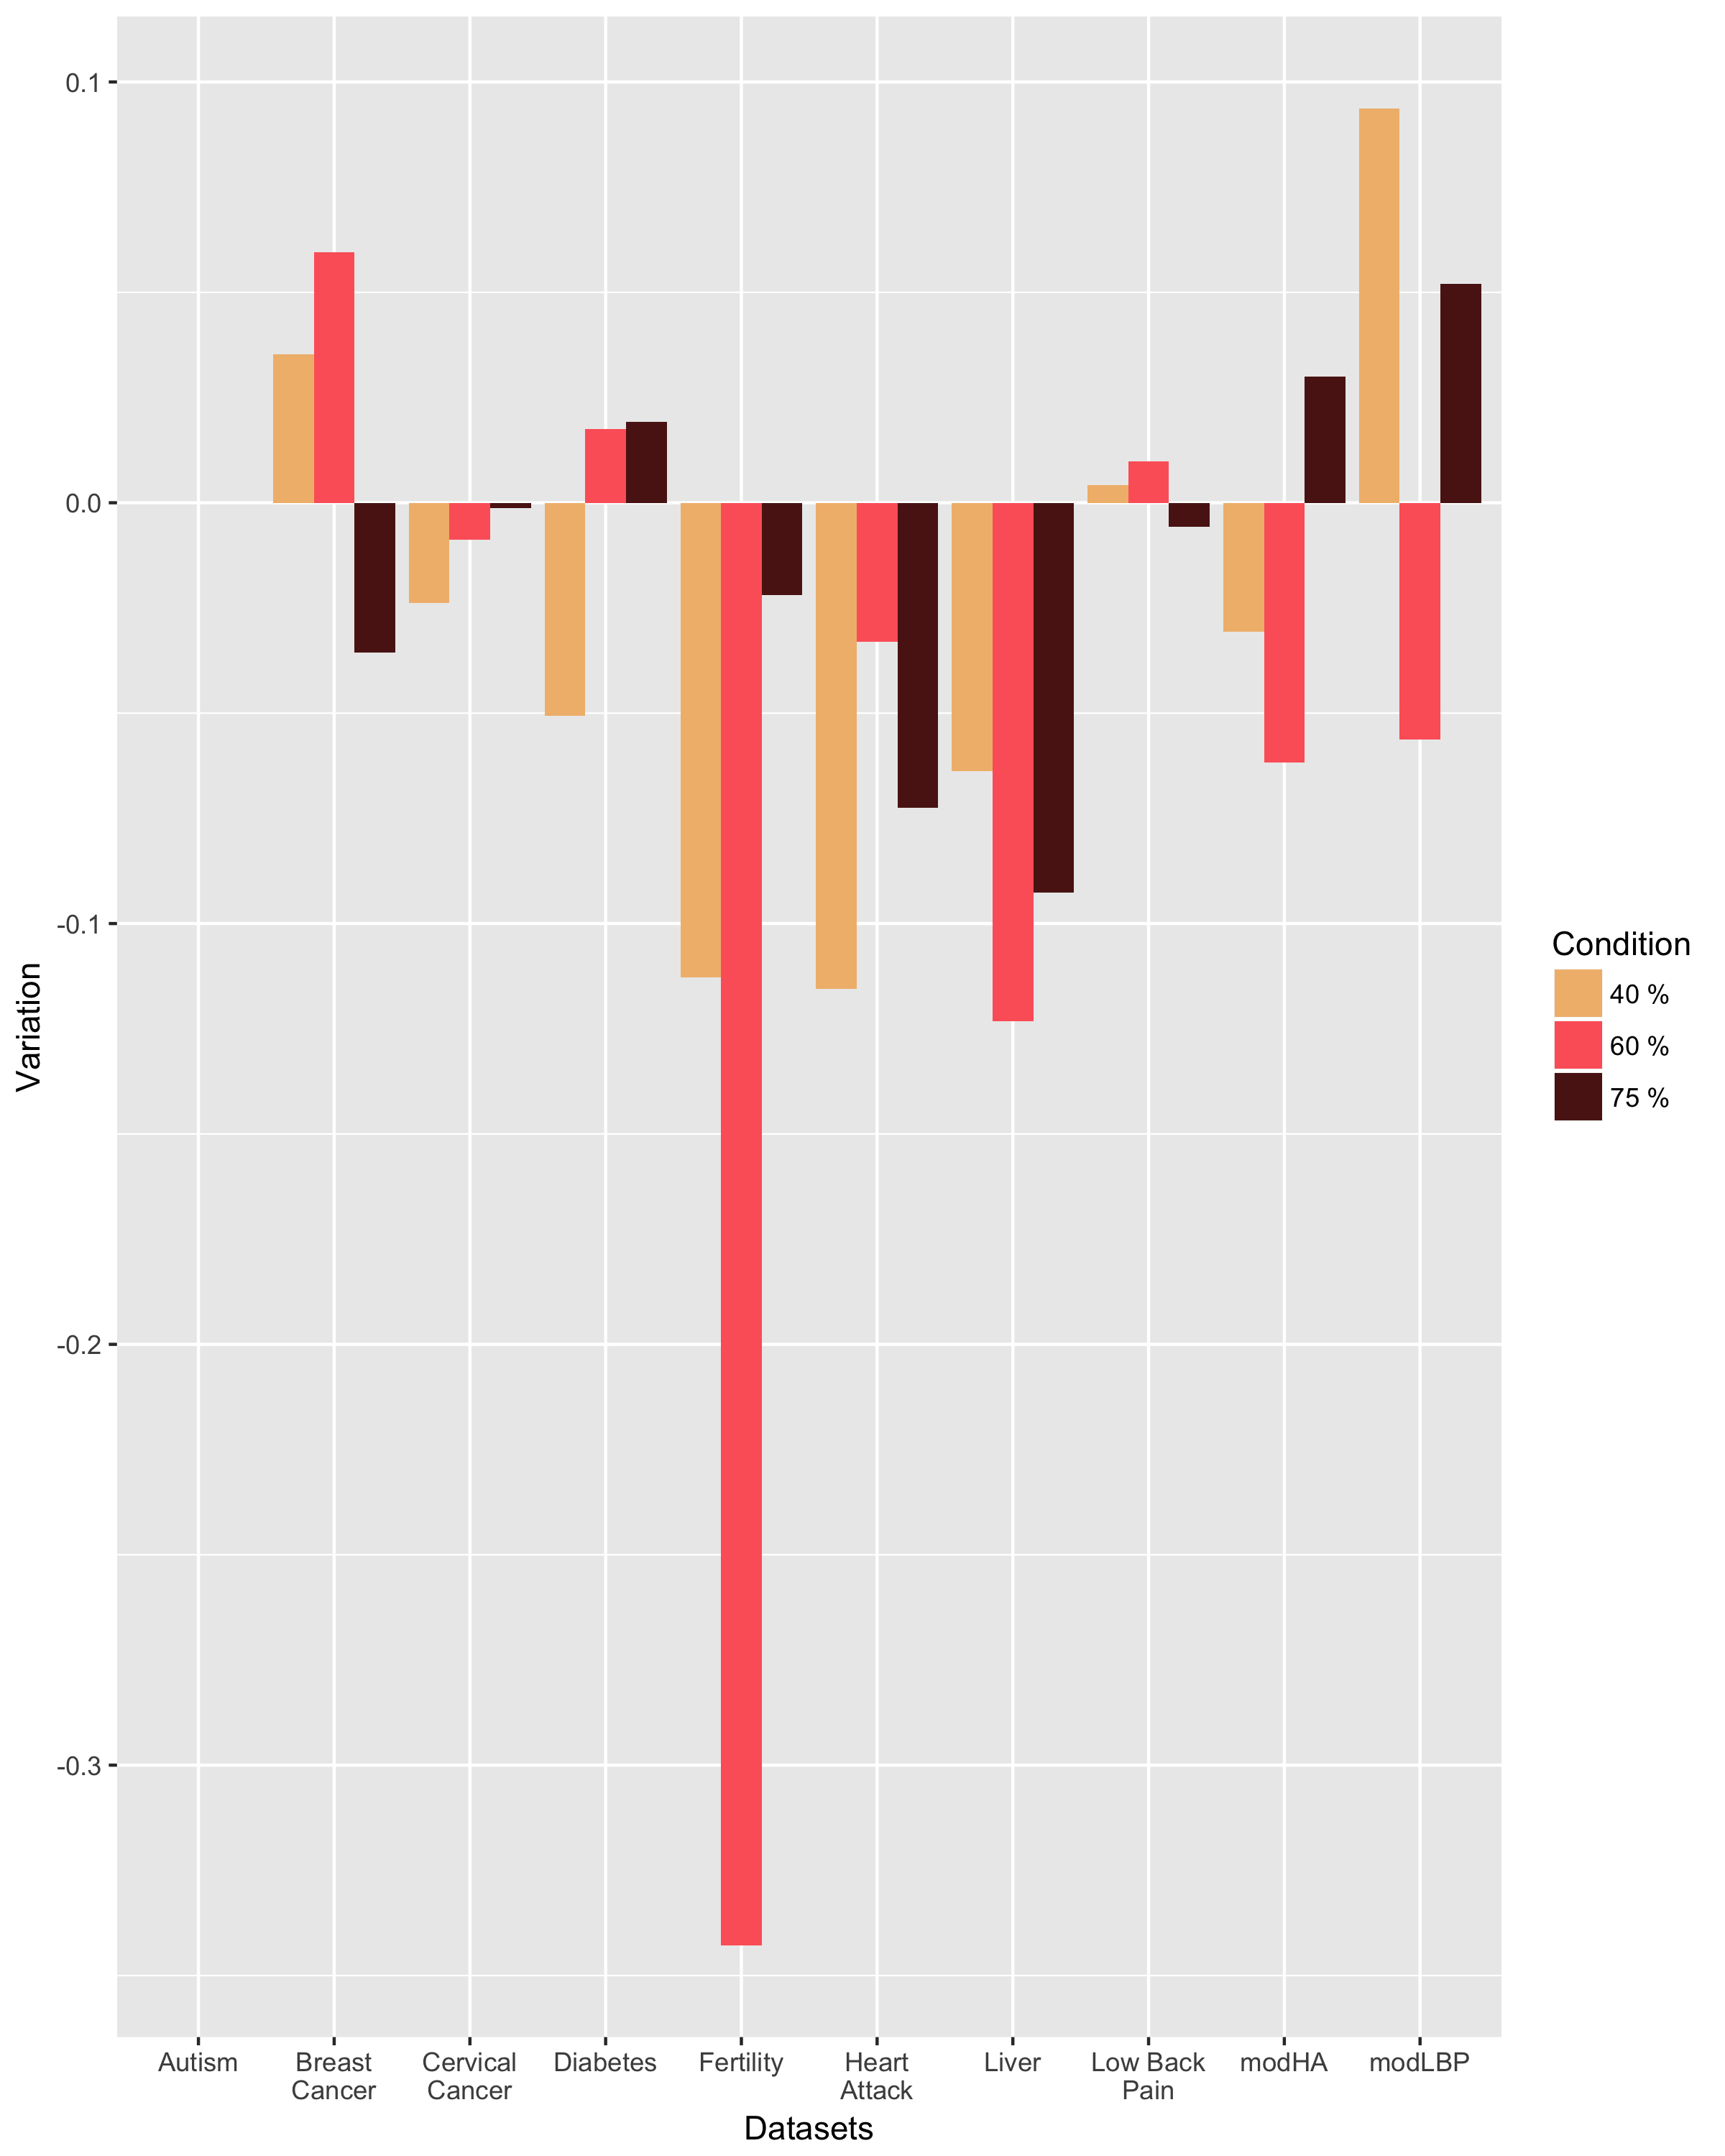
\includegraphics[width=0.9\textwidth]{ThesisTemplate/usingLatex/chapter5Images/AccuVariationUnderBySets.png}
    \caption{Variation of the accuracy value for the three under-sampling conditions compared to the baseline established in Experiment 1 for all studied datasets.}
    \label{fig:my_label}
\end{figure}

Figure 5.1 shows the variations in accuracy observed when 75\%, 60\% and 40\% of the majority class was retained.
Overall the effect is that of a decrease in accuracy when under-sampling of the  majority class is applied, though the effect is slight (less than 0.15 variation for most datasets, except for the Diabetes dataset where the accuracy is greatly affected when under-sampling occurs).\newline



\begin{figure}[!htbp]
    \centering
    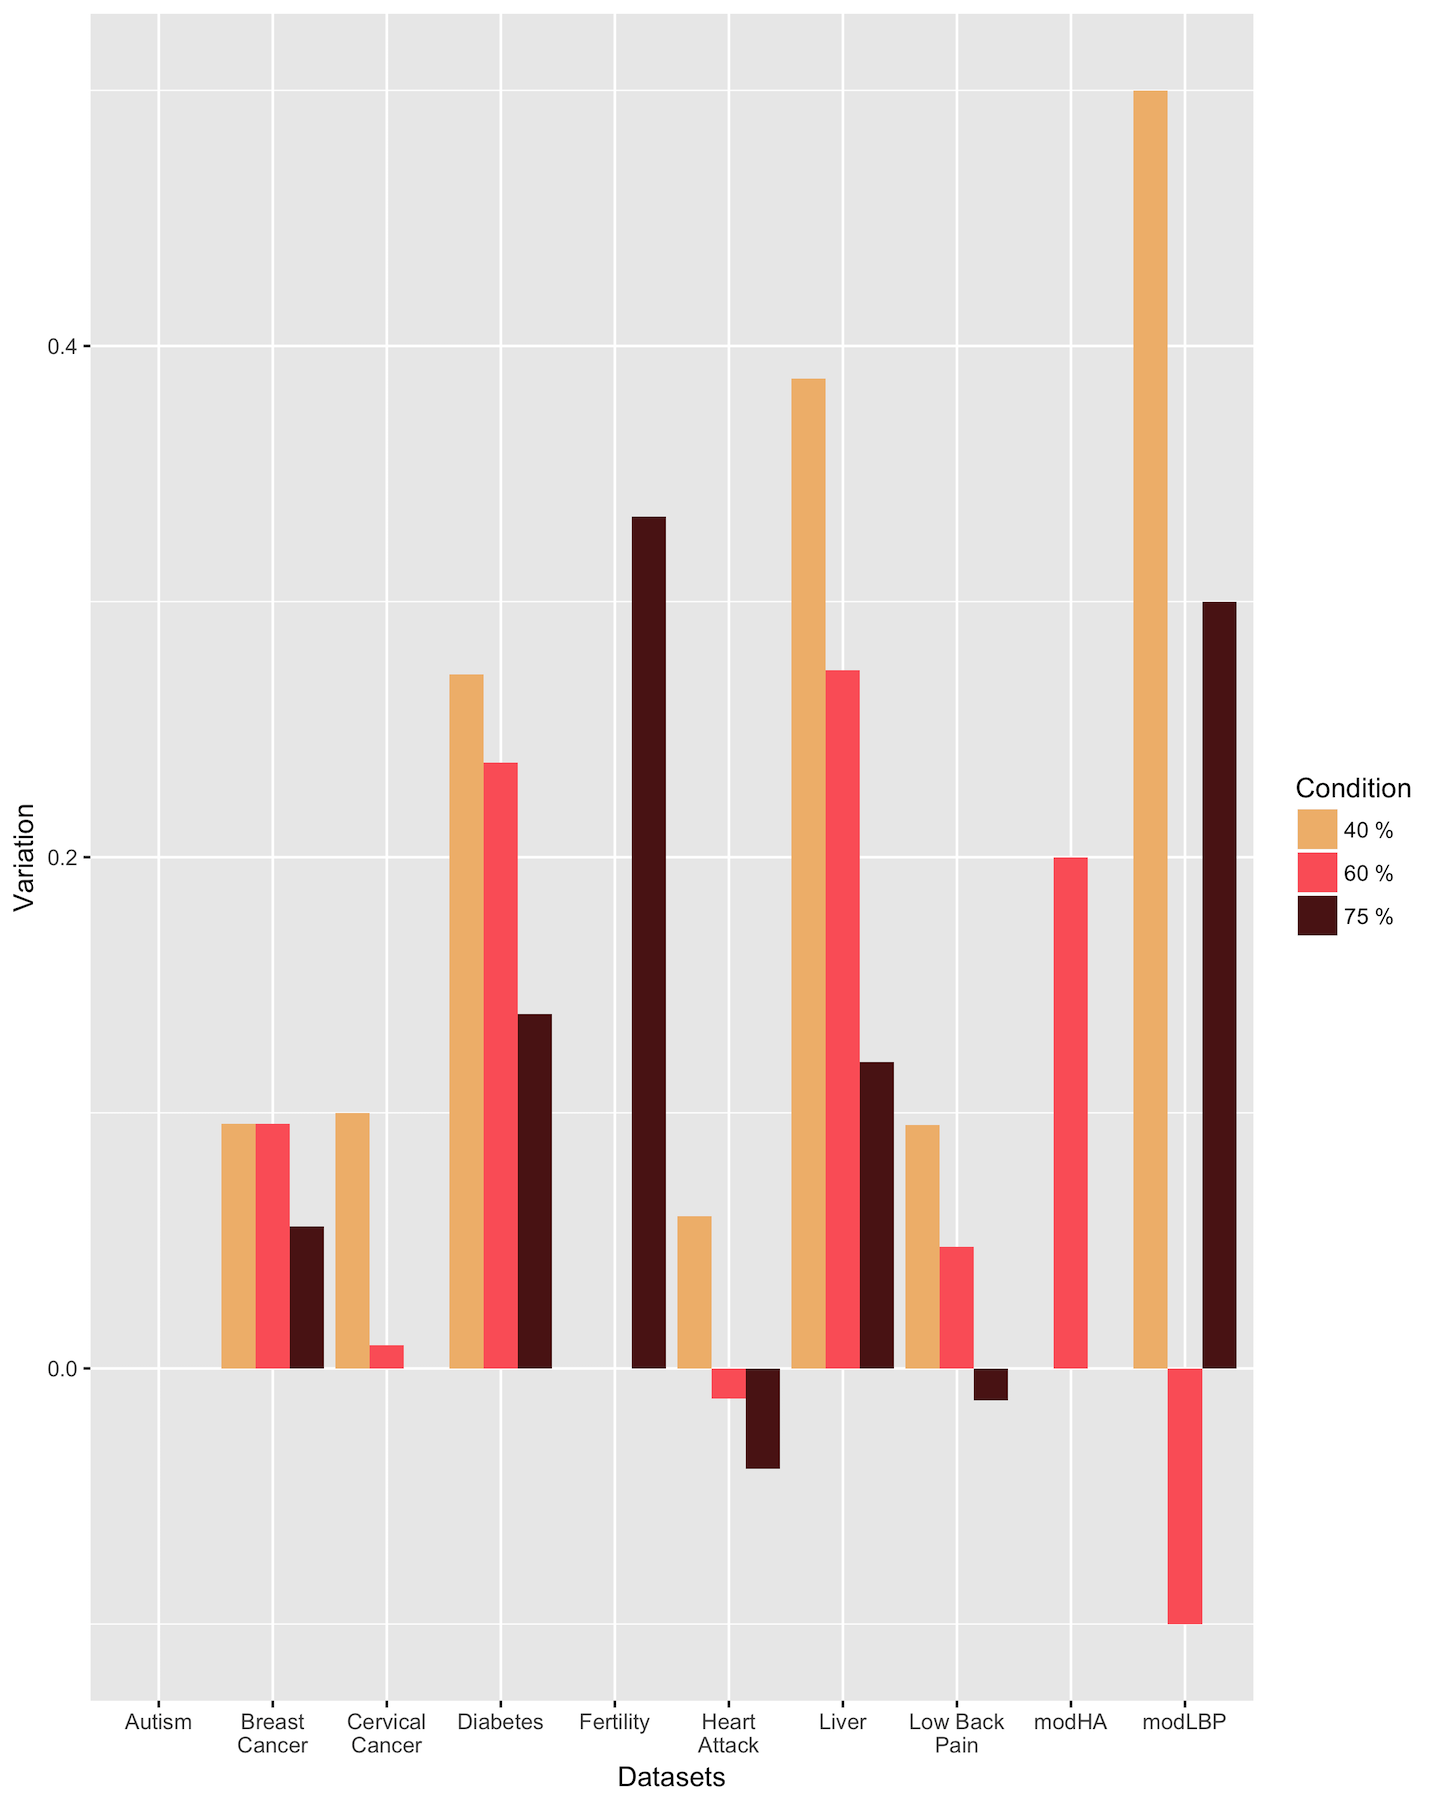
\includegraphics[width=0.9\textwidth]{ThesisTemplate/usingLatex/chapter5Images/SensiVariationUnderBySets.png}
    \caption{Variation of the sensitivity value for the three under-sampling conditions compared to the baseline established in Experiment 1 for all studied datasets.}
    \label{fig:my_label}
\end{figure}
Figure 5.2 shows the variations in sensitivity observed when   75\%, 60\% and 40\% of the majority class was retained. The overall effect is that sensitivity increases when under-sampling is applied; The trend is that the more of the majority class has been discarded, the more the sensitivity increases, the highest observed increase is 0.4.\newline



\begin{figure}[!htbp]
    \centering
    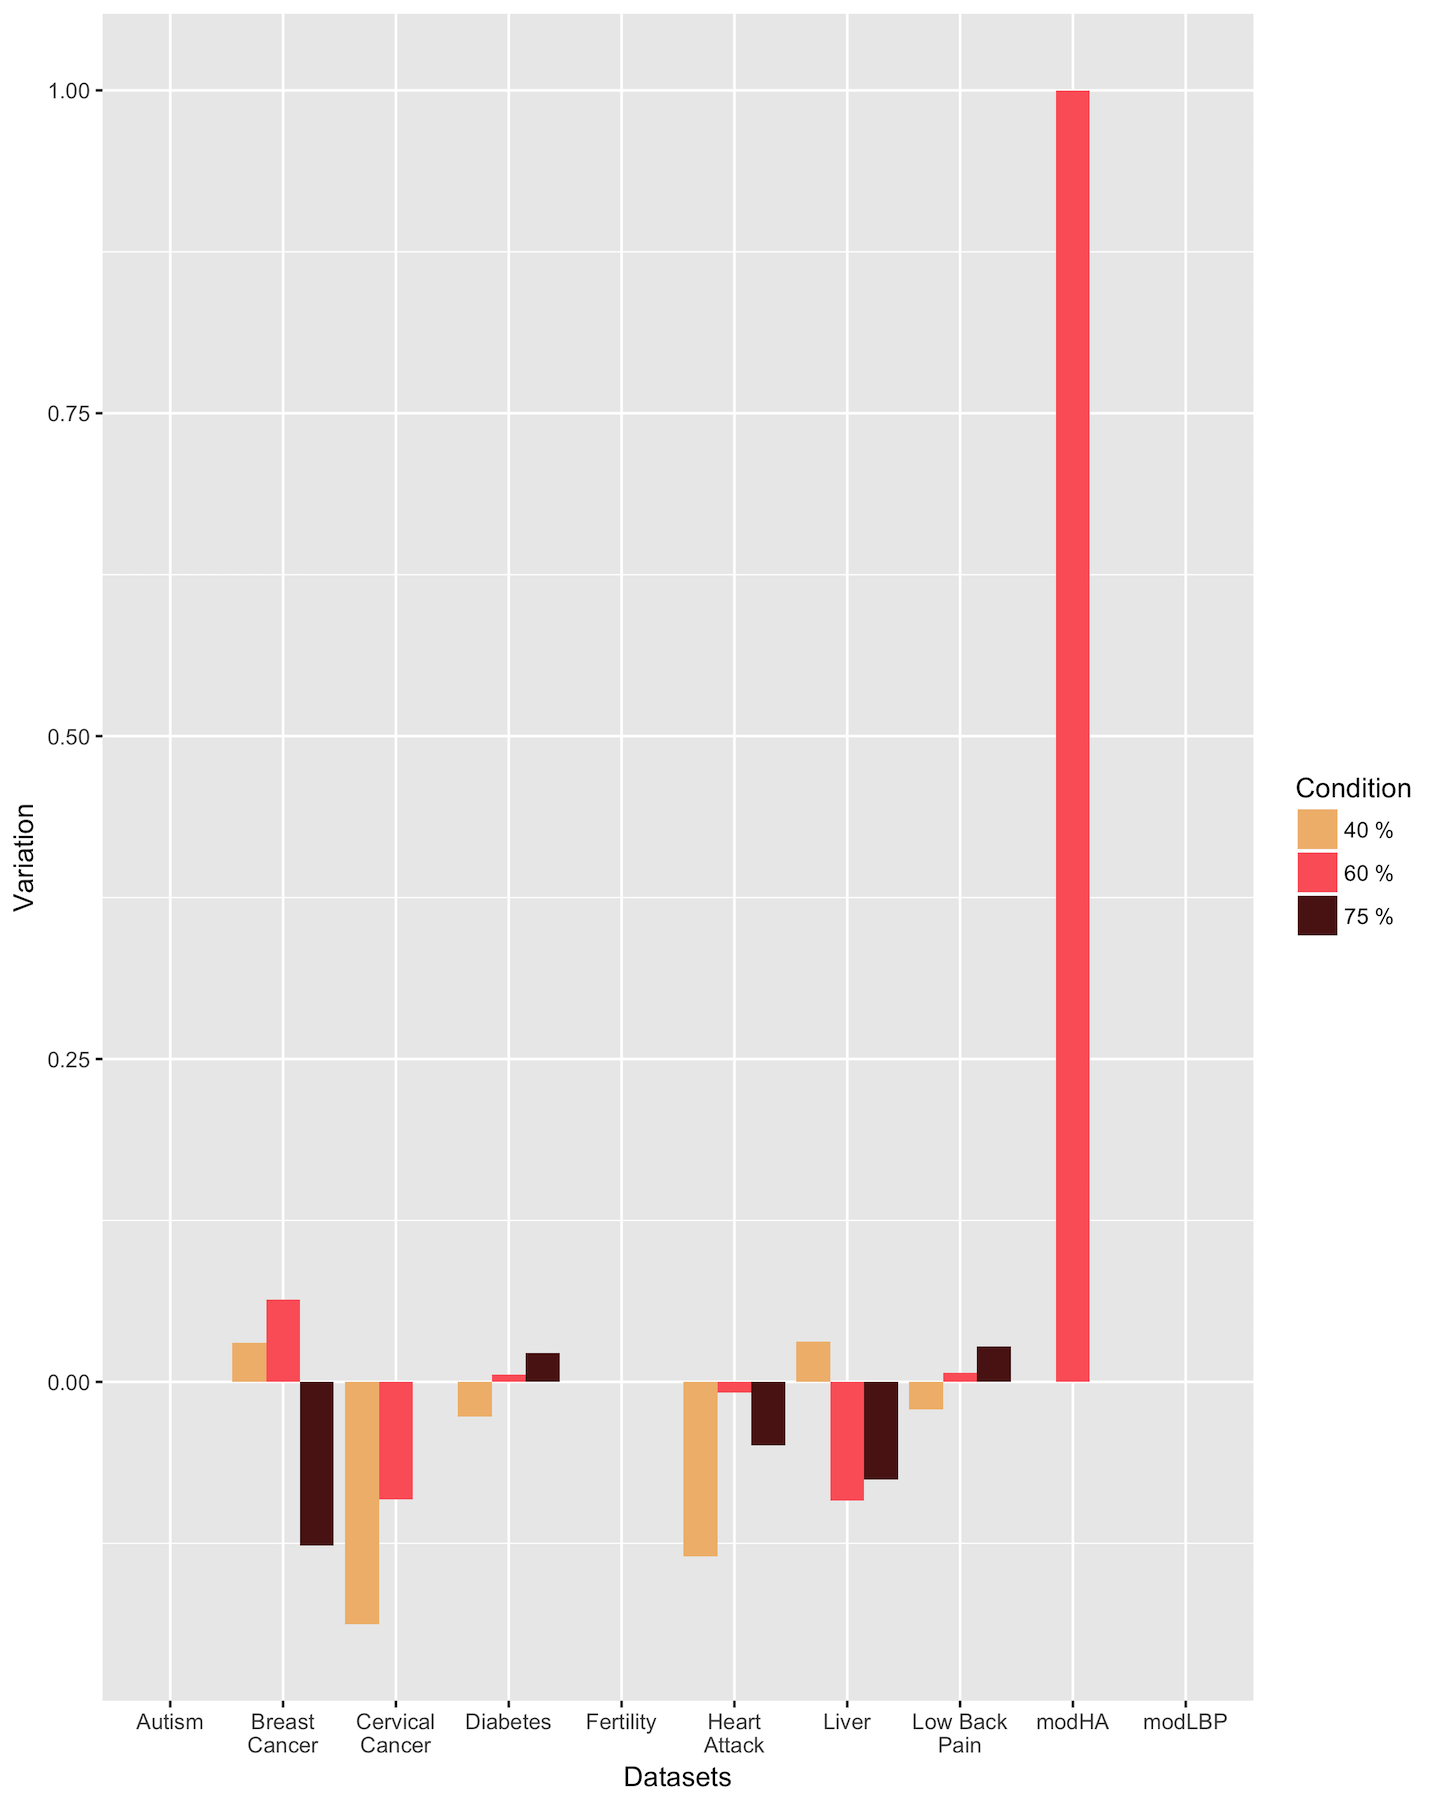
\includegraphics[width=0.9\textwidth]{ThesisTemplate/usingLatex/chapter5Images/PreciVariationUnderBySets.png}
    \caption{Variation of the precision value for the three under-sampling conditions compared to the baseline established in Experiment 1 for all studied datasets.}
    \label{fig:my_label}
\end{figure}

Figure 5.3 shows the variations in precision observed when 75\%, 60\% and 40\% of the majority class was retained. In general, precision is reduced by under-sampling, particularly if the proportion of the majority class to be discarded is large, though the effect remains light (maximum reduction is 0.19) In one case (modified Heart Attack dataset), the precision value is greatly increase when 60\% of the majority class is retained, though that effect is not consistent with what is observed on the other datasets.\newline

\begin{figure}[!htbp]
    \centering
    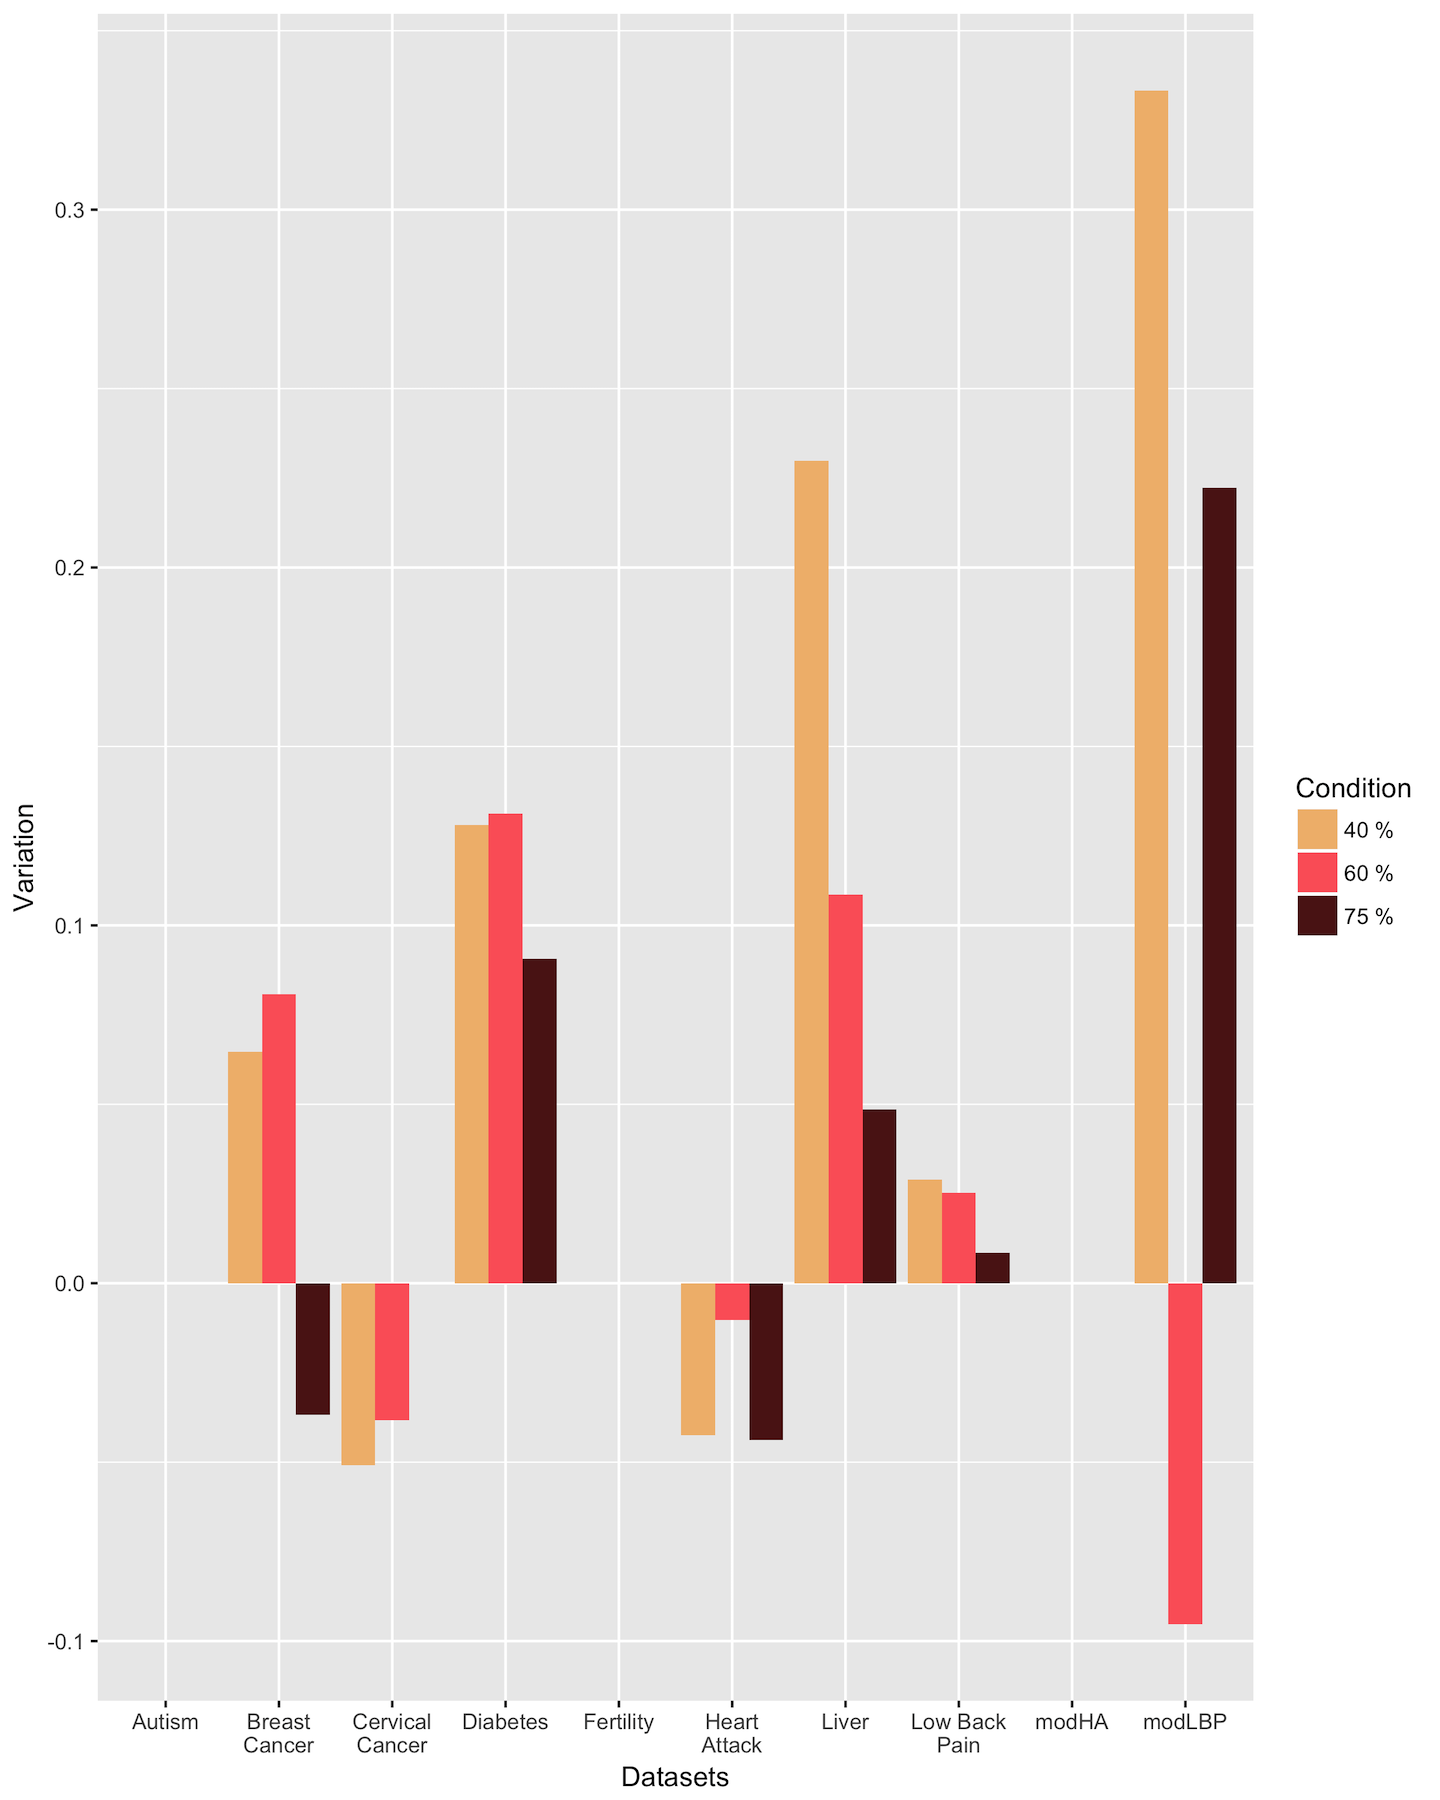
\includegraphics[width=0.9\textwidth]{ThesisTemplate/usingLatex/chapter5Images/F1VariationUnderBySets.png}
    \caption{Variation of the F1 score value for the three under-sampling conditions compared to the baseline established in Experiment 1 for all studied datasets.}
    \label{fig:my_label}
\end{figure}

Figure 5.4 shows the variations in F1 score observed when 75\%, 60\% and 40\% of the majority class was retained. In general the F1 score increases with the increased proportion of discarded majority class. The F1 score is partly dependent on both precision and sensitivity, but as previously discussed sensitivity tends to increase when the proportion of majority class discarded increases while precision decreases when the proportion of majority class discarded increases but to a lesser extent; thus the overall effect on the F1 score is that it increases as the proportion of majority class discarded increases.\newline

\subsection{Over-sampling the minority class (SMOTE)}
Over-sampling was carried out using the smote() function of R (see script Experiment3.R).\newline
The smote() function was applied to the datasets Fertility, modified Heart Attack and modified Low Back Pain with different parameters (see Chapter 4.3.2). 

\begin{table}[!htbp]
\centering
\begin{tabular}{lrrrr}
  \hline
  \rowcolor{LightCyan}
Dataset & MajorityClass & MinorityClass & NewMajorityClass & NewMinorityClass \\ 
  \hline
AuSDf [1] & 353 & 140 & 280 & 280 \\ 
  BCDf [1] & 258 & 143 & 286 & 286 \\ 
  CCDf [1] & 573 &  29 &  58 &  58 \\ 
  DiabetesDf [1] & 362 & 178 & 356 & 356 \\ 
  HAPDf [1] & 131 &  76 & 152 & 152 \\ 
  LBPDf [1] &  71 & 147 & 142 & 142 \\ 
  LiverDf [1]& 297 & 113 & 226 & 226 \\ 
   \hline
subHAPDf [2]& 134 &   7 & 112 &  63 \\ 
  subLBPDf [2] &  72 &  10 & 160 &  90 \\ 
  \hline
FertDf [3] &  61 &  10 & 120 &  70 \\ 
   \hline
\end{tabular}
\caption{Class distribution of the training sets before and after smote() has been applied with the parameters [1]:perc.under =100, perc.over =200, k=4, [2]: perc.under =200, perc.over = 800, k=4, [3]: perc.under =200, perc.over = 600, k=4}
\end{table}

These datasets already contain a low number of observations,  particularly in the minority class so the the training test contained even less observations in the minority class. If the parameters used for the other datasets are applied to Fertility, modified Heart Attack and modified Low Back Pain, not enough majority class points are retained compared to the newly generated minority class observations, thus leading to a large amount of data loss.\newline
The new class distribution obtained for these datasets after SMOTE was applied is shown in table 5.5.\newline
With these parameters, a new class distribution was achieved of 1:1 ratio majority:minority for the the Autism, Breast Cancer, Cervical Cancer, Diabetes, Heart Attack, Low Back Pain and Liver datasets. The new ratio observed for modified Heart Attack, modified Low Back Pain and Fertility is 1.7:1. \newline


\begin{table}[!htbp]
\centering
\begin{tabular}{lrrrr}
  \hline
  \rowcolor{LightCyan}
Dataset & Accuracy & Sensitivity & Precision & F1Score \\ 
  \hline
AuSDf & 1 & 1.00 & 1.00 & 1.00 \\ 
  BCDf & 0.9464 & 0.96 & 0.92 & 0.94 \\ 
  CCDf & 0.9688 & 1.00 & 0.56 & 0.71 \\ 
  DiabetesDf & 0.7412 & 0.72 & 0.66 & 0.69 \\ 
  HAPDf & 0.8966 & 0.90 & 0.82 & 0.86 \\ 
  LBPDf & 0.8152 & 0.81 & 0.91 & 0.86 \\ 
  LiverDf & 0.6821 & 0.85 & 0.49 & 0.63 \\ 
  subHAPDf & 0.9474 & 0.67 & 0.50 & 0.57 \\ 
  subLBPDf & 0.7500 & 0.50 & 0.25 & 0.33 \\ 
  FertDf & 0.7241 & 0.50 & 0.12 & 0.20 \\ 
   \hline
\end{tabular}
\caption{Performance metrics obtained after smote has been applied to the training sets}
\end{table}

Table 5.6 shows the results obtained for the performance metrics for Random Forest after SMOTE was carried out.\newline
As previously noted, the results obtained for the Autism dataset are unchanged when SMOTE has been applied to the dataset.\newline
Table D.5 in the Appendix shows the variations observed for each of the metrics when compared to the baseline established in Experiment 1 and they are represented on figure 5.5.\newline

\begin{figure}[!htbp]
    \centering
    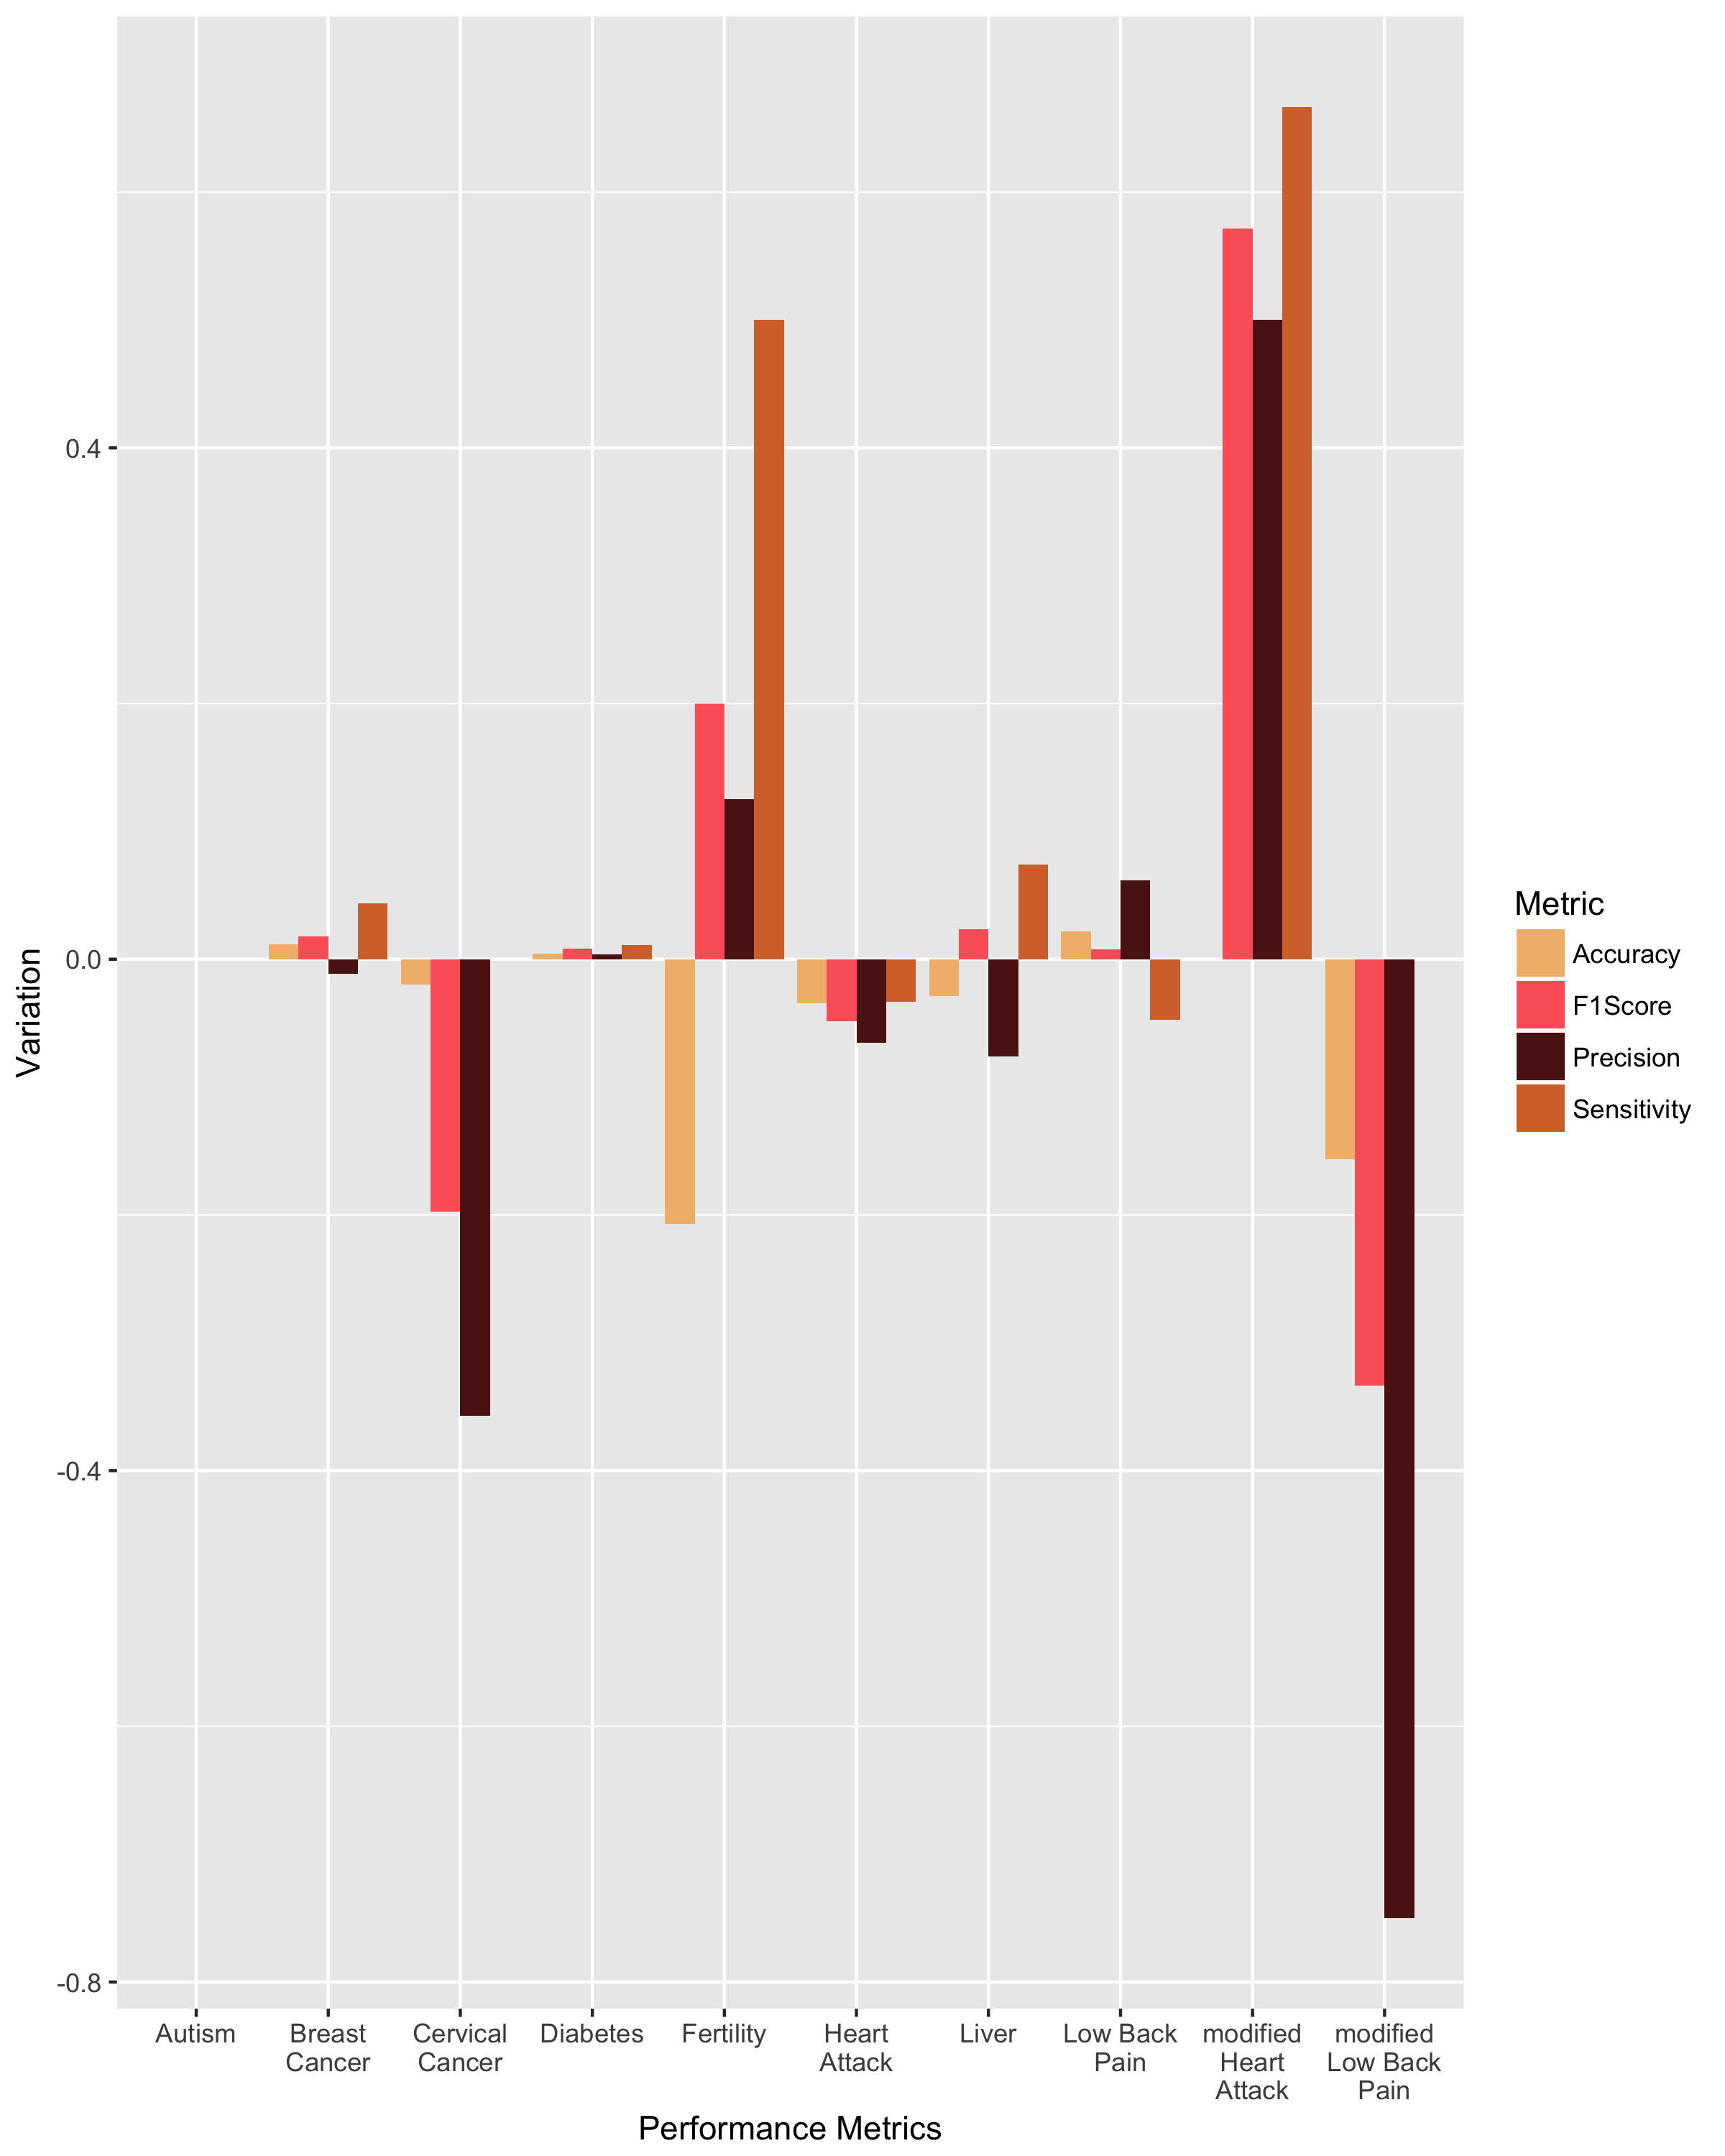
\includegraphics[width=0.9\textwidth]{ThesisTemplate/usingLatex/chapter5Images/OverVariations.png}
    \caption{Observed variations for all measured metrics after SMOTE compared to the baseline established in Experiment 1 for all studied datasets.}
    \label{fig:my_label}
\end{figure}

Figure 5.5. shows that the effect of SMOTE being applied to the training set was minimal for the Breast Cancer and Diabetes datasets while the largest effect was observed for the Fertility, Cervical Cancer,  modified Heart Attack dataset and modified Low Back Pain.\newline 
For the Cervical Cancer and modified Low Back Pain the use of SMOTE on the training set resulted in an important decrease in precision and F1 score, though sensitivity was unchanged.\newline
For both the Fertility and modified Heart Attack dataset, the sensitivity, precision and F1 score increased.\newline
A decrease in Accuracy can be noted for Cervical Cancer and Liver datasets but it is increased for Breast Cancer and unchanged for the others.\newline
Sensitivity is increased for Breast Cancer, Cervical Cancer, Diabetes and Heart Attack datasets but decreased for Low Back Pain and Liver datasets. Precision is increased for Breast Cancer, Cervical Cancer, Low back Pain and Liver datasets but decreased for Diabetes and Heart Attack. Finally the F1 score is increased for Breast Cancer, Diabetes and Liver. It is unchanged for Heart Attack and it decreases for Cervical Cancer and Low Back Pain.\newline
For the modified Heart Attack and modified Low Back Pain datasets, the Accuracy was decreased in both cases. Sensitivity was increased for modified Heart Attack but unchanged for the modified Low Back Pain. Precision was increased for modified Heart Attack but decreased for modified Low Back Pain and the F1 score increased in both cases.\newline
In this case of the Fertility dataset, although the overall accuracy of the algorithm was reduced, the sensitivity was increased and both precision and F1 score were given a value (when Random Forest is applied to the dataset without prior modification both precision and F1 returned a non-value).\newline


\section{Discussion}
The data obtained in Experiments 1, 2 and 3 were combined to produce the graph shown in figure 5.6 with a view to show the the effects of under-sampling and over-sampling by SMOTE on all the data sets side by side. The Autism dataset was not represented on this figure as none of the metrics studied here were affected by any of the data manipulation.\newline

\begin{figure}[!htbp]
    \centering
    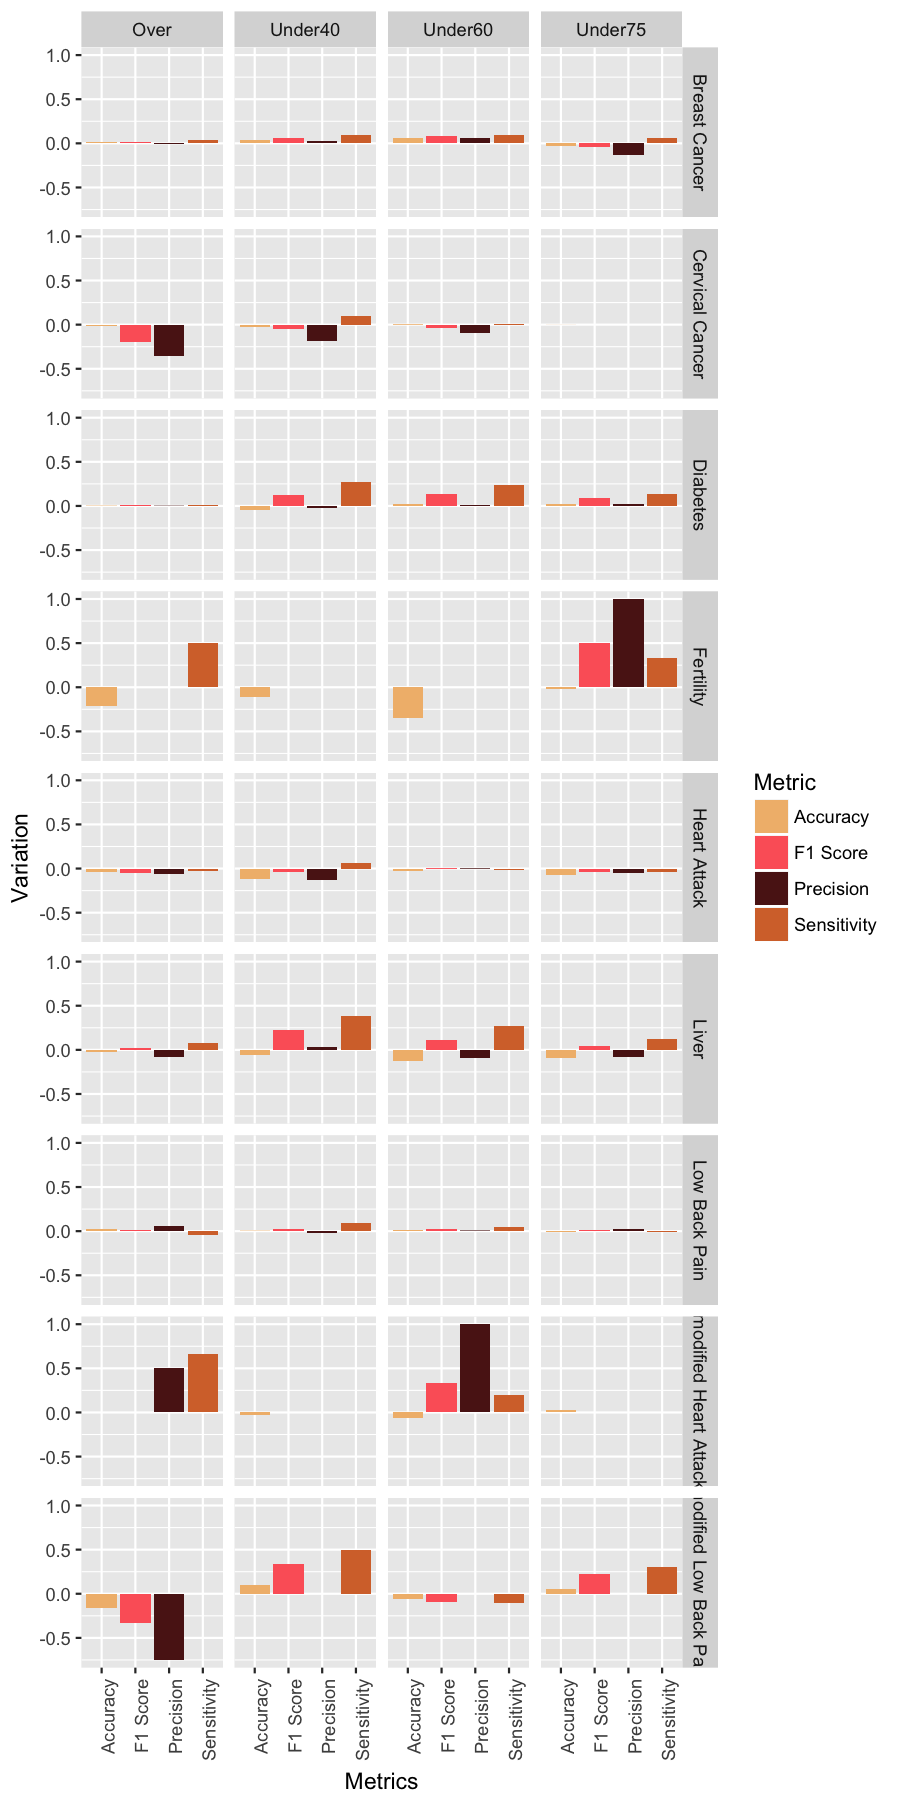
\includegraphics[width=0.8\textwidth]{ThesisTemplate/usingLatex/chapter5Images/AllMetricsPortrait.png}
    \caption{Observed variations for all measured metrics after SMOTE compared to the baseline established in Experiment 1 for all studied datasets.}
    \label{fig:my_label}
\end{figure}

When taking into account the class distribution of the datasets before and after SMOTE was applied, or before and after under-sampling was applied, there doesn't seem to be a pattern of effect linked to the new class ratio. For those datasets that achieved a 1:1 ratio after SMOTE, the results were not similar to those obtained after under-sampling which achieved the same ratio (discarding 40\% of the majority class achieved this for all but the Cervical Cancer and Fertility datasets). \newline 
Overall SMOTE did not produce large changes in overall accuracy, compared to the effects seen with under-sampling. The metrics most affected by both SMOTE and under-sampling sensitivity and precision. Generally speaking, SMOTE did not enhance the metrics measured in this project for the datasets considered.\newline
In the case of the Cervical Cancer dataset, the decrease in Precision and F1 score while accuracy increased slightly and sensitivity remained unchanged can be explained by the large reduction of the majority class compared to the original training set after SMOTE was carried out (see table 5.5). The reduced number of observations in the majority class means there are less cases for the model to learn what a negative case is, hence reducing the precision (increase in the number of false positive). This trends is also observed in the results from the under-sampling experiments where the larger reduction of majority class yielded lower precision scores, while sensitivity was increased, though only when the new class ratio was reduced from 21:1 to 8.4:1 (a 2.5-fold reduction).\newline
It is difficult to identify a discernible trend in the effect caused by under-sampling or over-sampling across all datasets and there seem to be a strong data-dependent effect. Generally, under-sampling reduces accuracy and precision while increasing sensitivity. The F1 score is either increased or decreased depending on the scope of variation of both precision and sensitivity. A large increase in F1 score suggests that both precision and sensitivity increase.\newline
SMOTE only improved the performance of the Random Forest algorithms in two cases: Fertility and modified Heart Attack where a 7- and 9-fold increase in positive data points was created, respectively, although the class ratio was 1.7:1 rather 1:1. This suggests that balancing the class ratio is not the only objective which should be aimed for when using SMOTE, providing many more data positive case points for the algorithm to train on, especially in smaller sample sets may be as important. The fact that the effect of SMOTE on algorithm performance is most noticeable for those datasets that had very low numbers of total and positive observations and where the parameters of the smote() function were different than those used for the other datasets suggests that SMOTE is most effective when applied to small datasets with low number of positive observations and the perc.over parameter needs to be set to a number that will more than doubled the positive cases.\newline
In the case of under-sampling, the biggest improvements to the performance of Random Forest for these algorithms was seen when 60\% of the majority class was discarded. This condition resulted in an increase in sensitivity in 7/9 cases. This however caused accuracy to decrease in all cases and precision decreased in 5/9 cases. When under-sampling was carried out in smaller proportion, accuracy and precision was still reduced but sensitivity did not increase to the same extent or for as many cases (6/9 cases when 75\% of the majority class was retained).\newline
Figure 5.6 also shows that for a given dataset, under-sampling provides a better improvement of performance than over-sampling by SMOTE, which has also been observed by other authors \citep{Rekha:2019uu}.
Statistical analysis was carried out on the values obtained from Experiments 1 and 2. An independent t-test and a Mann-Whitney test was carried out using the software SSPS to evaluate the significance of the variations for each metrics between the baseline (no under-sampling) and each under-sampling condition and over-sampling condition.\newline
The output files from SSPS can be found in the github repository and in the appendix. Table 5.7. shows the 2-tail t-test sigma values obtained for each independent t-test and table 5.8 shows the results of the Mann-Whitney test. All tests were carried out with and without the values for the Autism dataset as these remained unchanged in all experiments and may have affected the results of the t-test.\newline
The only sigma values inferior to 0.05 (i.e. showing statistical significant difference between the means) is seen for the sensitivity metric after SMOTE and while retaining the values obtained for the Autism dataset (independent t-test but not Mann-Whitney). This is most likely caused by the sharp increase in sensitivity seen for the Fertility and modified Heart Attack datasets.\newline
All other values are inferior to 0.05, which means that the observed differences are not significant. Importantly the statistics may not be accurately representing the results since the datasets show great variations in their structure and it may not be appropriate to calculate means for the metrics obtained for the 10 studied datasets since there appear to be a strong data-dependent effect on algorithm performance. Additionally, the samples for each test is small as only 10 datasets were analysed and in some cases the precision or F1 score values were not available, further reducing the number of available cases to be considered. A more extensive analysis with a larger number of datasets could potentially yield statistically significant results.\newline

\begin{table}[!htbp]
\centering
\begin{tabular}{*9c}
  \hline
  \rowcolor{LightCyan}
Condition &\multicolumn{2}{c}{Accuracy} &\multicolumn{2}{c}{Sensitivity} &\multicolumn{2}{c}{Precision}&\multicolumn{2}{c}{F1.Score}\\
  \hline
           & [A] & [B] & [A] & [B] & [A] & [B] & [A] & [B] \\
Under 40  &0.608& 0.581& 0.395 & 0.375 & 0.820 & 0.815 & 0.297 & 0.255 \\ 
  Under 60 &0.353& 0.318& 0.649 & 0.628 & 0.941 & 0.925 & 0.789 & 0.800 \\ 
  Under 75 &0.797&0.783 & 0.570 & 0.544 & 0.476 & 0.476 & 0.999 & 0.967 \\ 
  SMOTE &  0.396 & 0.303& 0.055 & 0.920  & .910 &0.975 & 0.320 & 0.545 \\
   \hline
\end{tabular}
\caption{2-tail t-test sigma values for independent t-test carried out on the results obtained for accuracy, sensitivity, precision and F1 score for each of the datasets. [A] Values obtained while keeping the results for the Autism dataset, [B] values obtained while removing the results obtained for the Autism dataset as they were unchanged in any of the conditions.}
\end{table}


\begin{table}[!htbp]
\centering
\begin{tabular}{*9c}
  \hline
  \rowcolor{LightCyan}
Condition &\multicolumn{2}{c}{Accuracy} &\multicolumn{2}{c}{Sensitivity} &\multicolumn{2}{c}{Precision}&\multicolumn{2}{c}{F1.Score}\\
  \hline
           & [A] & [B] & [A] & [B] & [A] & [B] & [A] & [B] \\
Under 40  &0.910& 0.860& 0.221 & 0.197 & 0.592 & 0.562 & 0.268 & 0.201 \\ 
  Under 60 &0.427& 0.354& 0.570 & 0.507 & 0.834 & 0.807 & 0.885 & 0.908 \\ 
  Under 75 &0.910&0.895 & 0.762 & 0.723 & 0.682 & 0.670 & 0.923 & 0.954 \\ 
  SMOTE &  0.545 & 0.480& 0.649 & 0.595  & 0.203 &0.177 & 0.307 & 0.266 \\
   \hline
\end{tabular}
\caption{Sigma values for Mann-Whitney test carried out on the results obtained for accuracy, sensitivity, precision and F1 score for each of the datasets. [A] Values obtained while keeping the results for the Autism dataset, [B] values obtained while removing the results obtained for the Autism dataset as they were unchanged in any of the conditions.}
\end{table}
 

\section{Conclusions}
The work described in this chapter fits in a wider context of research to assess the impact of class imbalance on the performance of algorithms such as recent work from Rekkha and colleagues \citep{Rekha:2019uu}. This is an ongoing area of research which should help define solutions to design and train algorithm for the best possible outcome.\newline
The results from the experiments carried out for this project show that there does not appear a "one-size-fit-all" solution to this problem and that the nature of the data and likely of the algorithm should be considered when attempting to improve the performance of an algorithm to be used on imbalanced data.\newline
It is also important to remember that when training an algorithm, if the distribution of the training set is markedly different from that of the testing sets, the performance of the algorithm could be affected \citep{Ling:2017jm}. Thus when applying either under-sampling or oversampling techniques to redress the class imbalance, the class distribution of the testing data should also be considered.\newline
The difficulties encountered with the Fertility dataset and the lack of obvious improvement in the performance of Random Forest when used with this dataset suggests that data-level solutions are not always sufficient in improving the performance of an algorithm and this will be discussed further in chapter 6.
The results of the experiments have shown that it is difficult to improve all metrics of algorithm performance and there is often a trade-off between accuracy, precision and sensitivity. In this set of experiments, there were only four  instances where both sensitivity and precision increased and only one case in which precision increased while sensitivity decreased. In 24 cases, sensitivity increased but precision remained constant or decreased and accuracy almost always decreased (27/32 cases).
In terms of real-life consequences, it would be less problematic for an individual to be told that they may suffer a condition and require more testing to confirm diagnostic (even if they are in fact confirmed to be healthy), than to be given a clean bill of health when they should have been identified as having a particular condition. As such, Sensitivity should be given more importance than Precision (though precision should still be viewed as important, particularly if computer-aided diagnostic is to help deliver more efficient healthcare) and Accuracy should remain high overall. This would suggest that best approach to improving algorithm performance over all the datasets used in this experiment would be to under-sample by discarding 25\% of the majority class only. This is an average outcome and as seen in the detailed graphs, for some datasets, discarding large amount of the majority class was necessary in order to correctly identify the sick patients at all (\textit{e.g.} Fertility dataset). \newline
